\chapter{Entwurfsmuster}

Für \glqq Chess of Duty\grqq{} wurde ein Observer-Pattern eingebaut.

\begin{balken}
    \tip
    \\
    Commit: \\
    \footnotesize \url{https://github.com/clemens1403/AdvSWE/commit/c04b243f87959c6f80f7d75ccf31cba30af50bd5}
\end{balken}

Ein Observer, auch als Beobachter bezeichnet, ist ein Entwurfsmuster in der Softwareentwicklung, das eine lose Kopplung zwischen Objekten ermöglicht. 
Mithilfe von Beobachtern können 1:N-Beziehungen hergestellt werden, wobei Änderungen an einem Objekt automatisch an alle abhängigen Objekte weitergegeben werden. Das Muster basiert auf zwei Komponenten:

\begin{itemize}
    \item Subject: Dieses Element im Code dient als Grundlage für die Beobachtung. Das Subjekt enthält eine Liste aller registrierten Beobachter und stellt Methoden für Registrierung, Entfernung und Benachrichtigung bereit. Sobald das Subjekt Änderungen erfährt, werden diese automatisch an alle registrierten Beobachter weitergegeben.
    \item Observer: Ein Beobachter implementiert die vom Subjekt definierte Schnittstelle, um Benachrichtigungen zu erhalten und auf Änderungen des Subjekts reagieren zu können.
\end{itemize}

Um das Schachspiel funktionsfähig zu machen, müssen alle grafischen Elemente regelmäßig gezeichnet werden. 
Dabei muss immer der aktuellste Zustand des Spiels dargestellt werden, der die Informationen aus der Anwendungsschicht entnimmt und über die Plugin-Schicht gezeichnet wird. 
Die Zeichner-Klassen müssen über Änderungen im aktuellen Spielstand informiert werden, sobald diese auftreten.

Im Folgenden werden der vorherige Stand und der nachherige Stand genauer beschrieben. 
Dabei werden UML-Diagramme für die visuelle Darstellung verwendet. 
Da die betrachteten Klassen im Kontext des gesamten Projekts ziemlich umfangreich sind und eine hohe Anzahl von Attributen und Funktionen aufweisen, wurde die Darstellung in den Diagrammen auf die wichtigsten Klassenbestandteile für die Implementierung des Observer-Musters reduziert.

\newpage

\section{Vor dem Entwurfsmuster}

Auch ohne die Implementierung des beschriebenen Beobachter-Musters war es erforderlich, den aktuellen Spielzustand aus der Spiellogikklasse an die Zeichnerklassen zu übergeben, um die grafische Oberfläche korrekt darzustellen. 
In Processing gibt es eine draw()-Methode, die zur Zeichnung von Grafiken verwendet werden kann. 
In dieser Methode werden die verschiedenen Zeichnerklassen koordiniert, um sicherzustellen, dass alle grafischen Elemente mehrmals pro Sekunde gezeichnet werden.

\begin{minipage}{\linewidth}
    \centering
    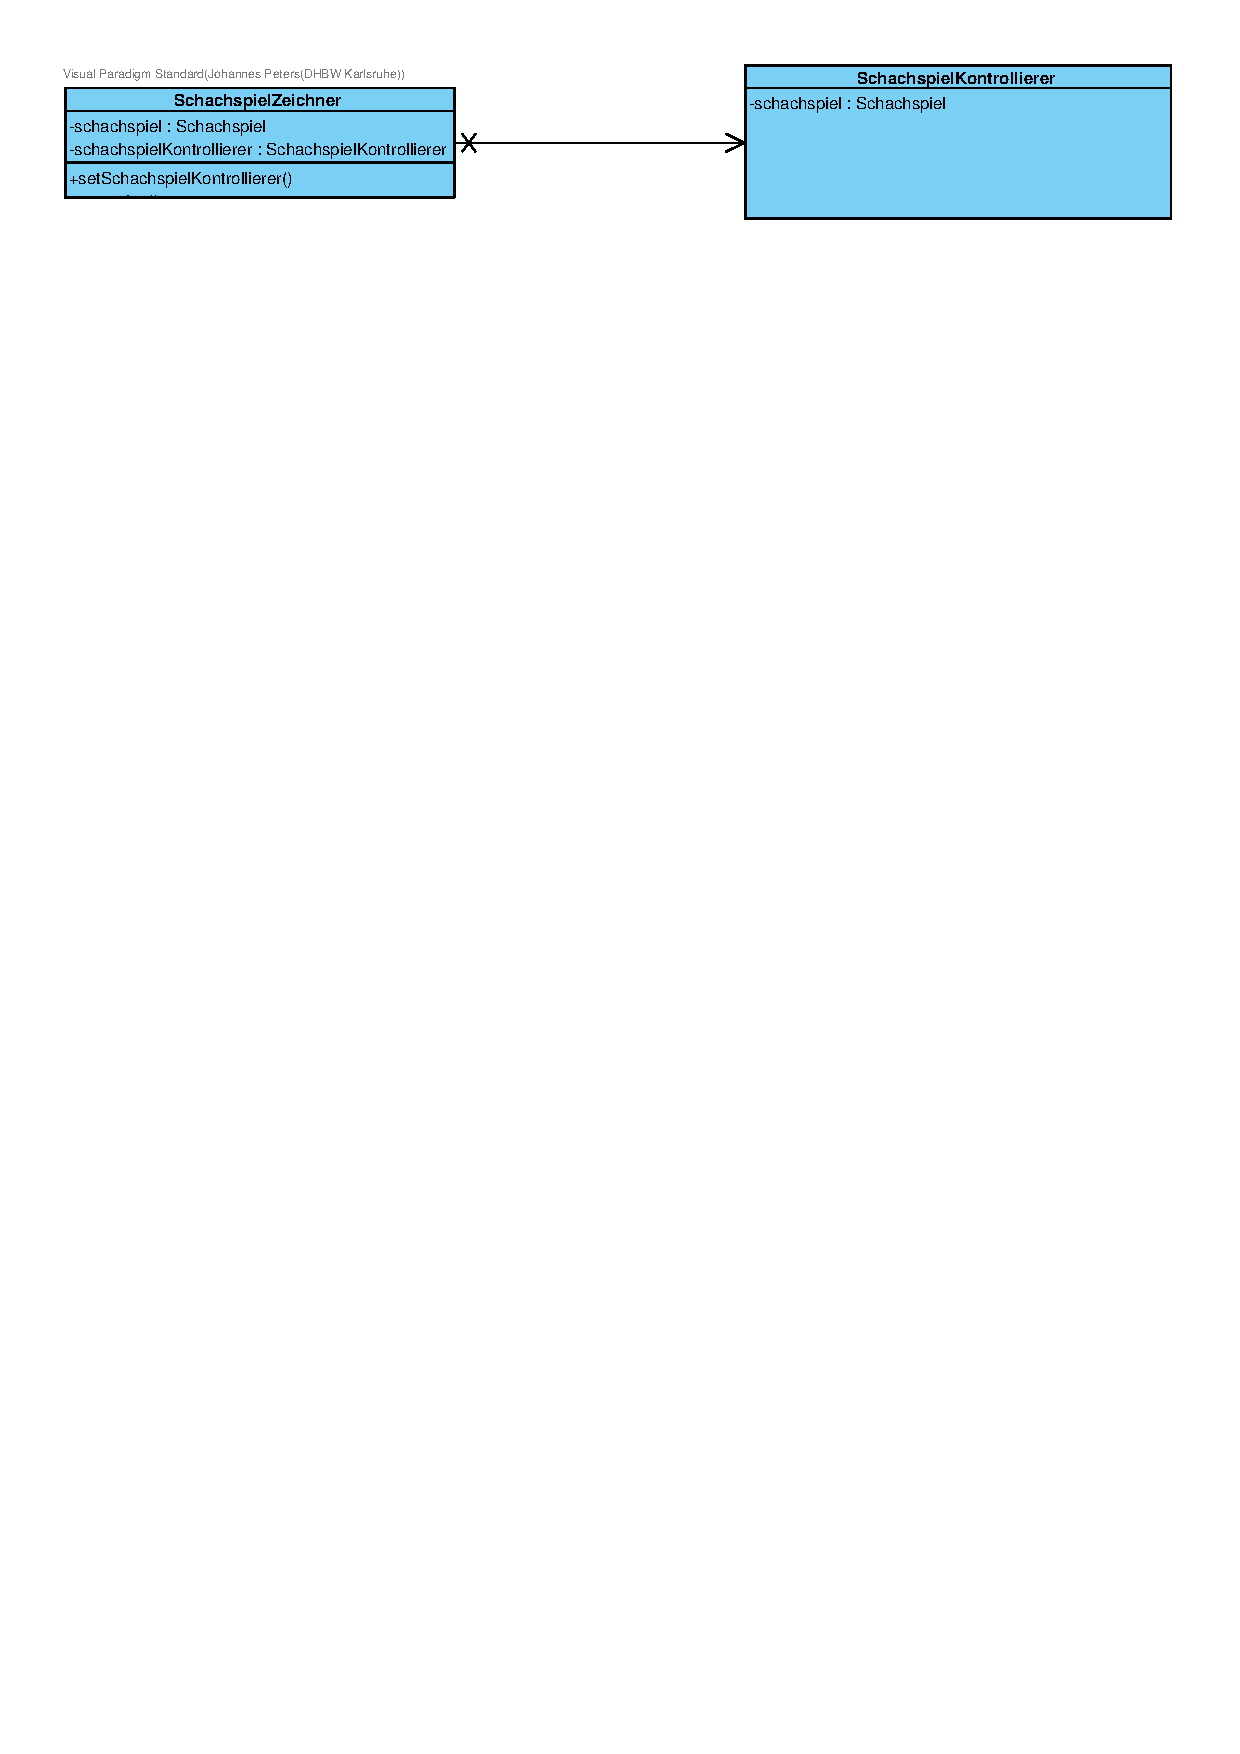
\includegraphics[scale=0.75, trim={0 25cm 0 0}]{Bilder/SWE_ohne_Observer.pdf}
    \captionof{figure}{Programmausschnitt ohne Observer-Pattern}
\end{minipage}

Ursprünglich wurde bei jedem Aufruf der draw()-Methode in der Zeichenklasse die Funktion \textit{setSchachspielKontrollierer} aufgerufen. 
Diese Funktion nimmt eine Instanz der Klasse \textit{SchachspielKontrollierer} entgegen und setzt sie als globale Variable in der Zeichnerklasse. 
Da jede übergebene Kontrollierer-Instanz die Variable \textit{Schachspiel} enthält, kann auch diese Variable lokal in der Zeichnerklasse gesetzt werden, um die Grafiken basierend darauf zu erstellen.

\newpage

\section{Mit dem Entwurfsmuster}

Um das Beobachter-Muster einzubauen, werden zwei zusätzliche Klassen benötigt: ein Interface für den Beobachter und ein Interface für das Subjekt. 
Im Rahmen des Programmentwurfs wurde ein Beobachter-Muster für das Attribut \glqq Schachspiel\grqq{} implementiert, um alle Änderungen zu registrieren.

Die Interfaceklasse für den Beobachter beschreibt die Methode \glqq aktualisiere()\grqq. 
Das Interface für das Subjekt enthält Methoden zum Registrieren, Entfernen und Benachrichtigen von Beobachtern. 
Diese Methoden müssen in den verschiedenen Klassen, in denen die Interfaces verwendet werden, überschrieben werden, um ihre Funktionalität genauer zu definieren.

\begin{minipage}{\linewidth}
    \centering
    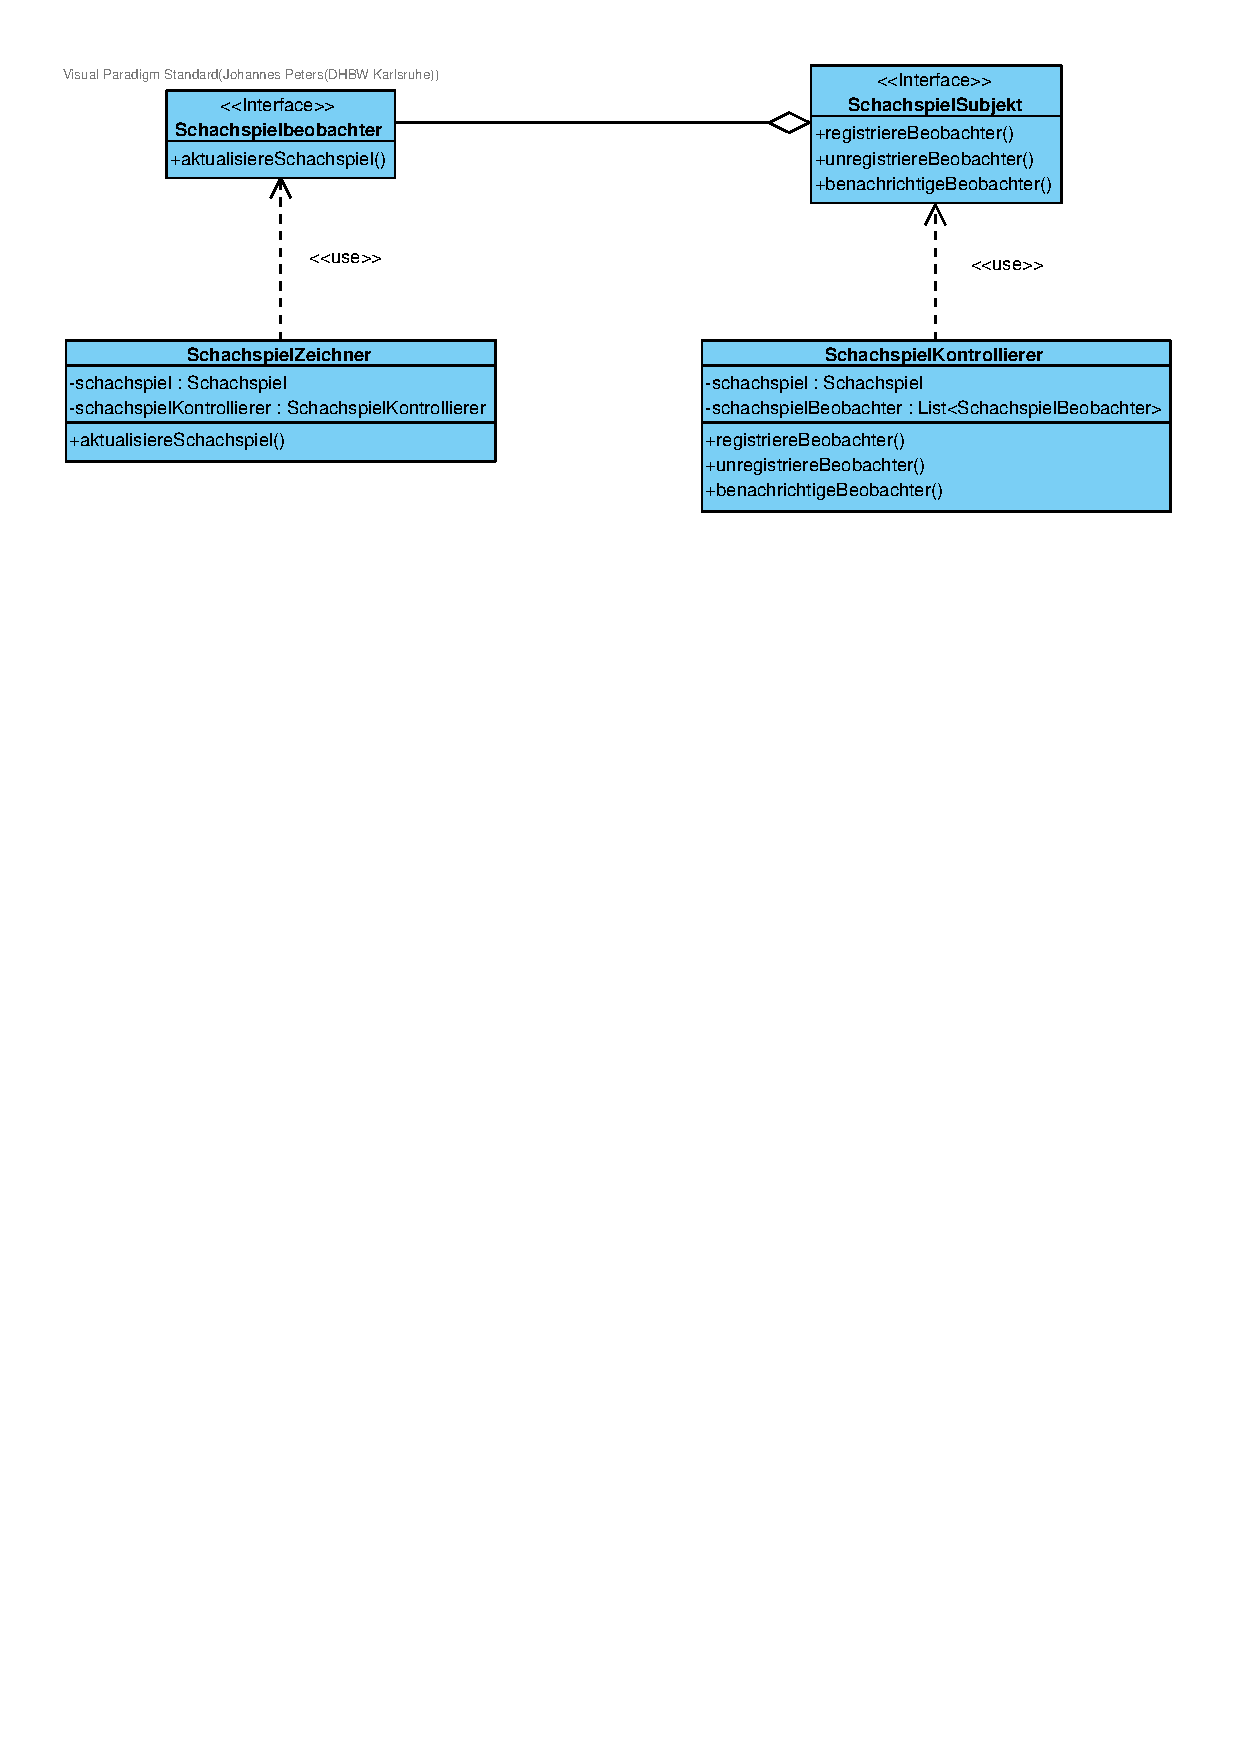
\includegraphics[scale=0.75, trim={0 20cm 0 0}]{Bilder/SWE_mit_Observer.pdf}
    \captionof{figure}{Programmausschnitt mit Observer-Pattern}
\end{minipage}

In der eigenen Implementierung des Schachprogramms verwendet die Zeichnerklasse \textit{SchachspielZeichner} das Beobachter-Interface. 
Die Klasse \textit{SchachspielKontrollierer}, die die Spiellogik steuert, implementiert das Subjekt-Interface. 
Da beide Klassen jeweils ein Interface verwenden, müssen die in den Interfaces beschriebenen Methoden überschrieben und implementiert werden.

Im Kontrollierer wird eine Liste von Beobachtern erstellt. 
Die Methoden \textit{registriereBeobachter()} und \textit{unregistriereBeobachter()}, die bereits im Interface definiert sind, verwalten die Beobachter-Instanzen, indem sie neue Beobachter hinzufügen oder bestehende Beobachter entfernen. 
Die Methode \textit{benachrichtigeBeobachter()} iteriert über die Liste der Beobachter und ruft für jeden Beobachter die Funktion \textit{aktualisiereSchachspiel()} auf.

In der Zeichnerklasse wird das Beobachter-Interface verwendet, und die Methode \textit{aktualisiereSchachspiel()} muss überschrieben werden. 
Diese neue Methode übernimmt die ursprüngliche Funktion der Methode \textit{setSchachspielKontrollierer}. 
Im Detail bedeutet dies, dass die neu geschriebene Methode durch den Aufruf des Beobachters einen neuen Kontrollierer erhält, aus dem die neueste Version von \textit{schachspiel} entnommen werden kann, sobald eine Änderung an diesem Attribut auftritt.

Wenn man die vorherigen und nachherigen Zustände betrachtet, könnte man denken, dass kein echter Mehrwert geschaffen wurde, sondern nur eine erhöhte Komplexität im Code entstanden ist. 
Doch dem ist nicht so. 
Anfangs wurde bei jedem Aufruf der draw()-Methode von Processing das Attribut \textit{schachspiel} an die Zeichnerklasse übergeben. 
Das Beobachter-Muster verhindert nun, dass das Attribut unnötigerweise mehrmals pro Sekunde neu gesetzt wird.
Mit dem eingebauten Beobachter für das Schachspiel-Attribut wird \textit{schachspiel} nur dann neu gesetzt, wenn es explizit vom Subjekt übergeben wird. 
Eine solche Übergabe wird nur ausgelöst, wenn sich das Schachspiel-Attribut tatsächlich ändert.
